% !TeX root = ../tfg.tex
% !TeX encoding = utf8

\chapter{ Planificación de trabajo y costes}\label{ap:apendicea}

\section{Planificación de trabajo}

Para poder llevar a cabo este proyecto se han identificado varios subproyectos que se han ido desarrollando a lo largo del año, siendo algunos de ellos dependientes del resultado de otros subproyectos. Se comienza haciendo una investigación y búsqueda bibliográfica del tema de la memoria, para proseguir con la redacción de la misma y, en paralelo, la realización de experimentos para comprobar algunos de los algoritmos expuestos, En la figura Fig~\ref{fig:gantt} se expone un diagrama de Gantt con la planificación seguida para cumplir los objetivos.

\begin{figure}[h]
    \centering
        \centering
        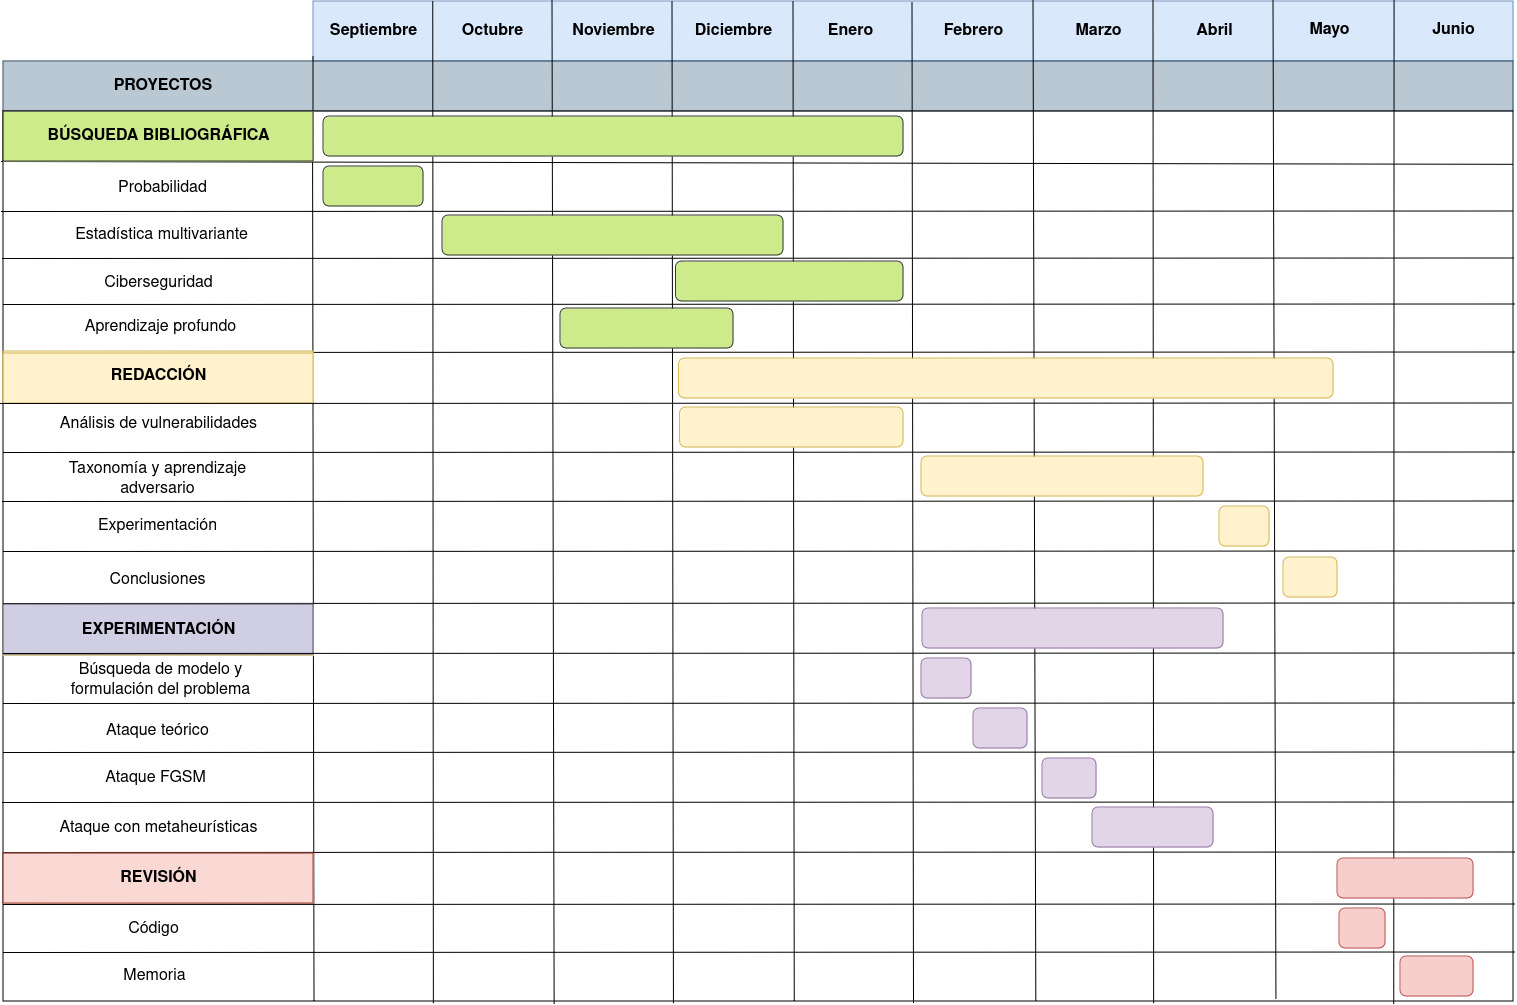
\includegraphics[width=\textwidth]{img/GanttTFG.jpg}
        \caption{Diagrama de Gantt para la planificación del trabajo}
        \label{fig:gantt}
\end{figure}

\newpage

\section{Presupuesto}

Se supone la siguiente situación: el alumno es un ingeniero contratado por una empresa, en este caso la Universidad de Granada, para realizar un proyecto como el expuesto en la memoria sobre robustez y seguridad de los modelos de aprendizaje profundo. Para estimar los gastos que debe realizar la universidad en el estudiante, se realiza un presupuesto donde se reune el coste de los materiales necesitados, licencias, sueldo del ingeniero y amortizaciones, entre otros. Para realizar de manera organizada este presupuesto, se usa una plantilla facilitada por el tutor, teniendo en cuenta lo siguiente:

\begin{item}
    \item El sueldo mensual debe sobrepasar el Sueldo Mínimo Interprofesional establecido por ley en España, el cual es $1134€$.

    \item Un sueldo medio de ingeniero es de $40$-$50 €$ brutos por hora. A la suma mensual se le debe aplicar el correspondiente IRPF y las cotizaciones.

    \item Este trabajo tiene una duración de $10$ meses aproximadamente.

    \item El ordenador se considera material inventariable, por lo que se puede amortizar a aproximadamente el $25 \%$.

    \item El IVA solo se aplica a los materiales usados, licencias y suministros consumidos, tales como electricidad. En el coste de personal se pagan impuestos según el IRPF y cotizaciones, por lo que el IVA no es aplicable.
\end{item}

El presupuesto general se expone en la tabla que aparecen en la figura Fig~\ref{fig:presupuesto}. Las tablas con el sueldo del ingeniero y los respectivos impuestos aparecen en las tablas en las figuras Fig~\ref{fig:pers1} y Fig~\ref{fig:pers2}, pudiendo observarse los porcentajes del IRPF en la tabla de la figura Fig~\ref{fig:irpf} y las cotizaciones en la tabla de la figura Fig~\ref{fig:cotiz}. Finalmente, en la tabla de la figura Fig~\ref{fig:amort} se puede contemplar una tabla con las amortizaciones asociadas al proyecto, teniendo en cuenta que se amortiza el ordenador (material informático) en cinco años.

\begin{figure}[h]
    \centering
        \centering
        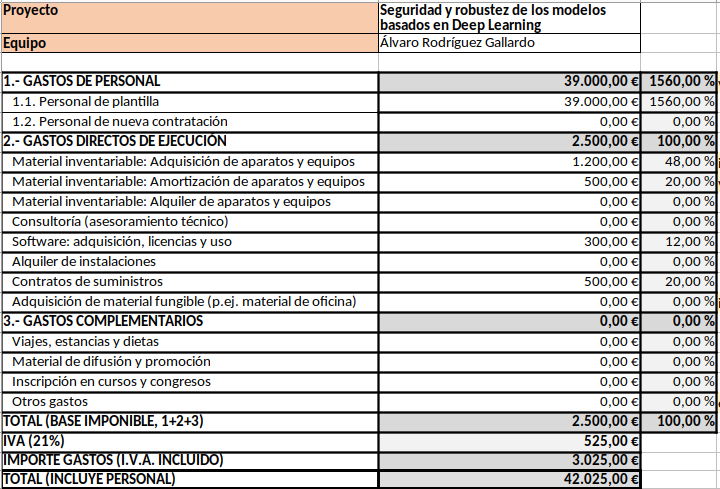
\includegraphics[width=\textwidth]{img/Presupuesto.png}
        \caption{Tabla general del presupuesto del proyecto}
        \label{fig:presupuesto}
\end{figure}

\begin{figure}[h]
    \centering
        \centering
        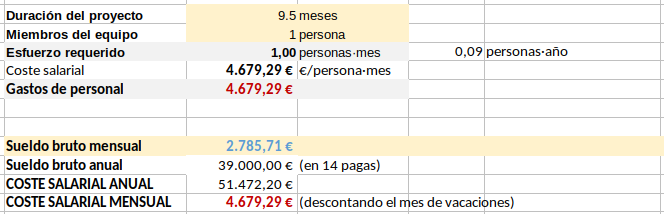
\includegraphics[width=0.6\textwidth]{img/Personal_1.png}
        \caption{Tabla con el sueldo bruto y costes del proyecto}
        \label{fig:pers1}
\end{figure}

\begin{figure}[h]
    \centering
        \centering
        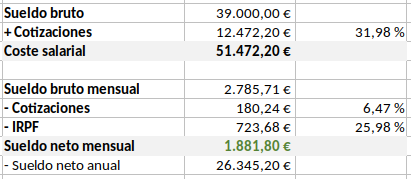
\includegraphics[width=0.6\textwidth]{img/Personal_2.png}
        \caption{Tabla con los impuestos aplicados y el sueldo neto}
        \label{fig:pers2}
\end{figure}

\begin{figure}[h]
    \centering
        \centering
        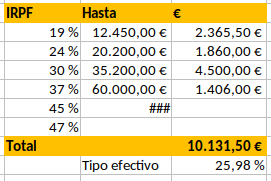
\includegraphics[width=0.6\textwidth]{img/Personal_IRPF.png}
        \caption{Tabla del IRPF}
        \label{fig:irpf}
\end{figure}

\begin{figure}[h]
    \centering
        \centering
        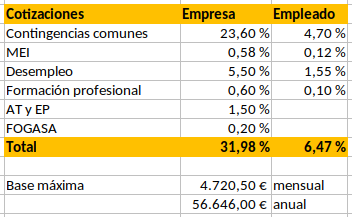
\includegraphics[width=0.6\textwidth]{img/Personal_cotizaciones.png}
        \caption{Tabla con las cotizaciones correspondientes}
        \label{fig:cotiz}
\end{figure}

\begin{figure}[h]
    \centering
        \centering
        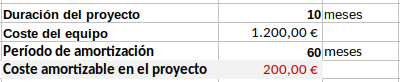
\includegraphics[width=0.6\textwidth]{img/Amortizaciones.png}
        \caption{Tabla de amortizaciones}
        \label{fig:amort}
\end{figure}